\chapter{Architettura}

\section{Struttura del sito}

\begin{figure}[ht]
      \centering
      \resizebox{\textwidth}{!}{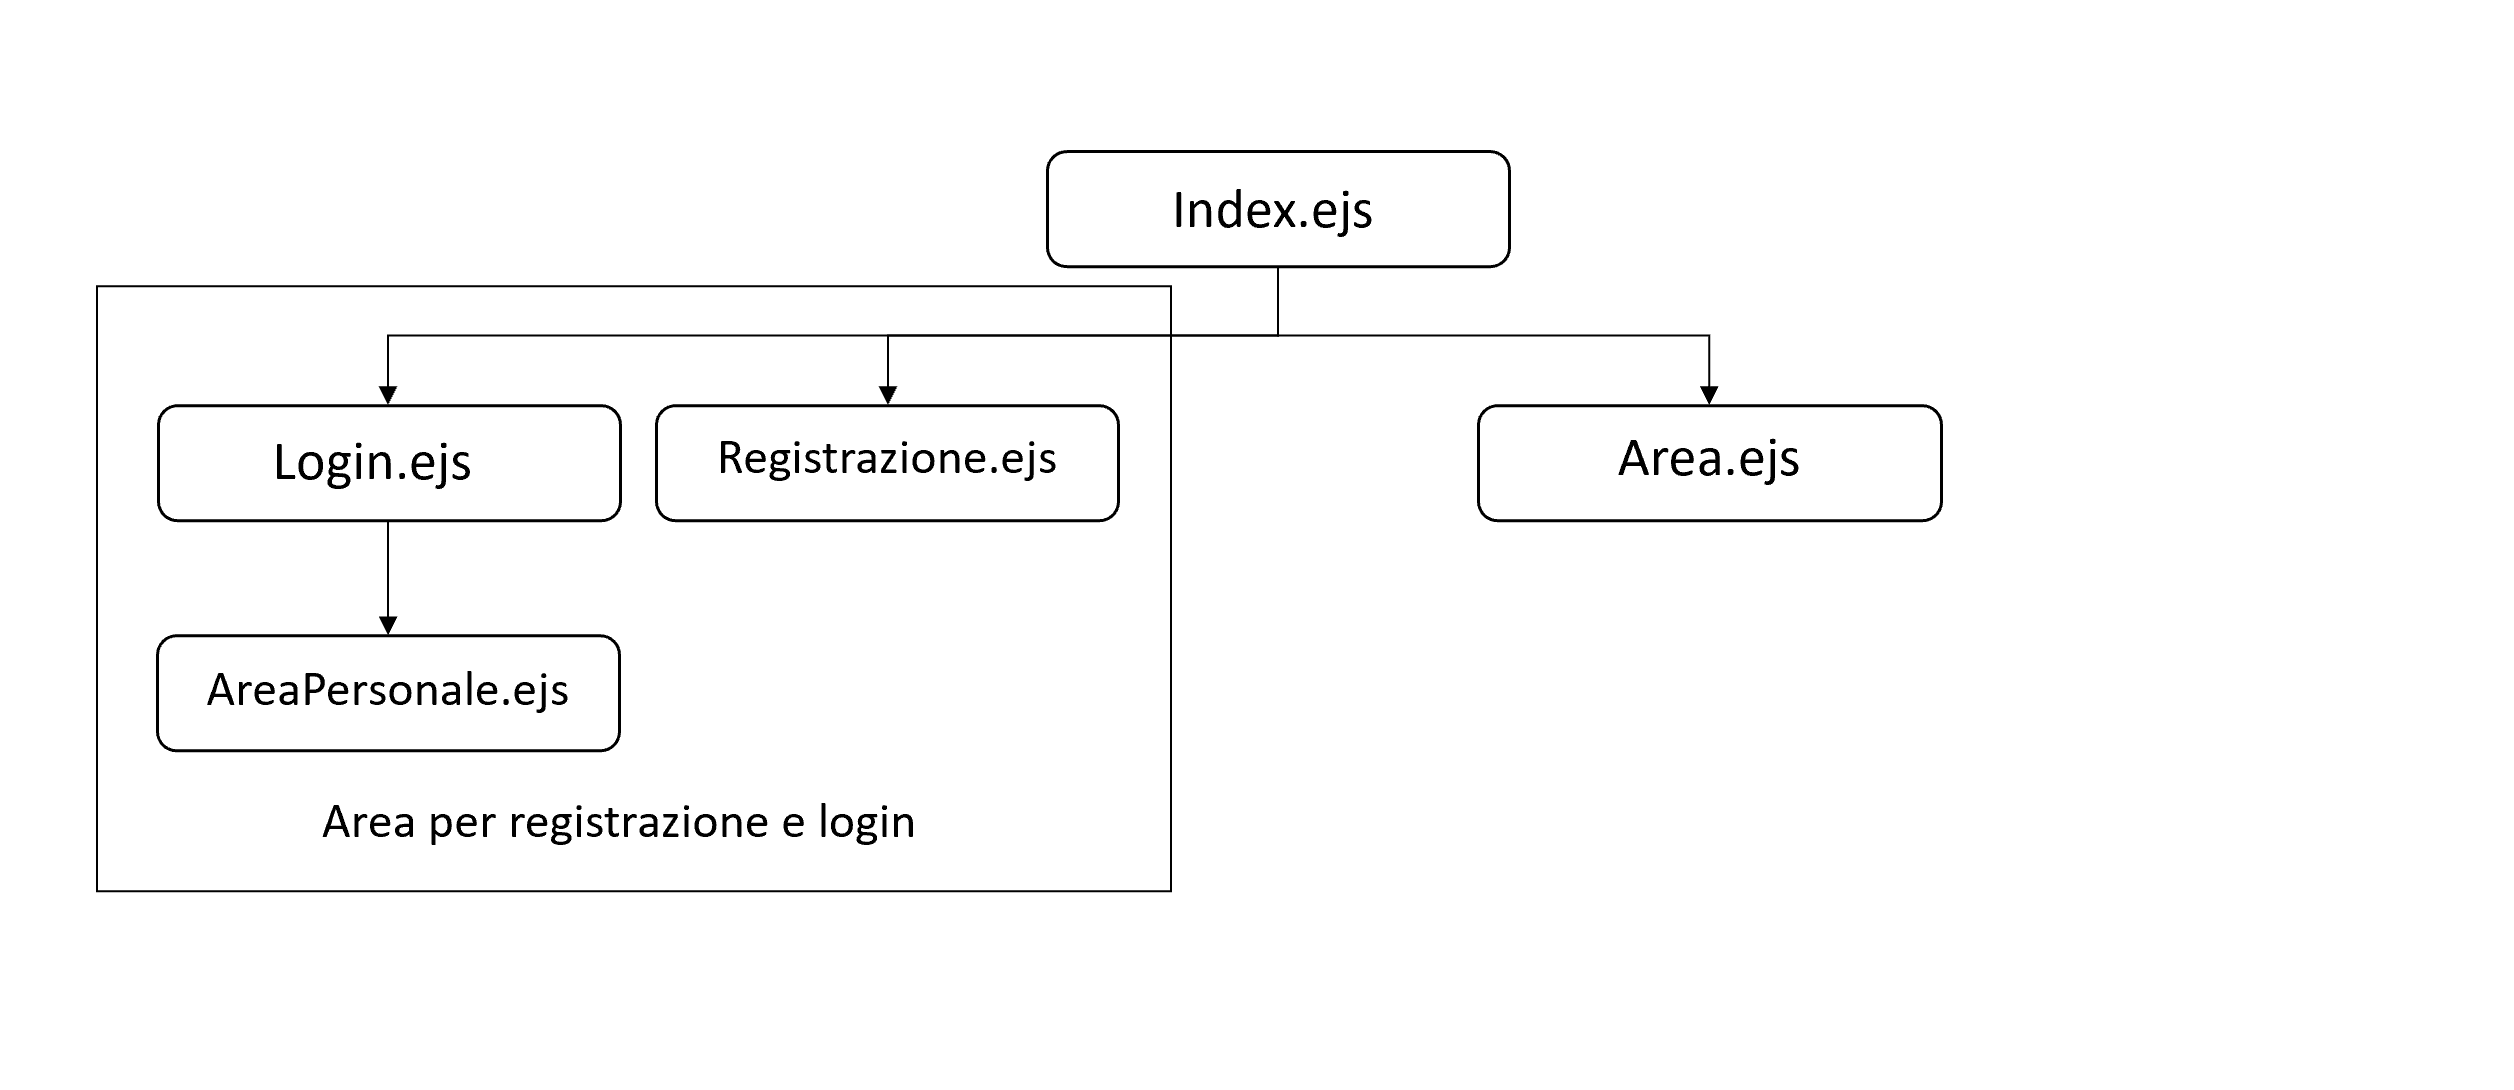
\includegraphics{img/architettura.png}}
      \caption{Architettura gerarchica delle pagine}
\end{figure}

Il punto di accesso al sito è pensato per essere costituito dall'index. Attraverso di essa sarà infatti
possibile accedere tramite uno o più passaggi a tutte le pagine del sito (la navigazione da una pagina all'altra rimane comunque
sempre disponibile attraverso la navbar, a prescindere da dove ci si trovi nel sito).

\vspace{5mm}

Per accedere alla pagina \emph{AreaPersonale.ejs} e a qualunque funzione che richieda di essere loggati,
sarà necessario aver effettuato realmente il login: in caso contrario, la richiesta verrà rifiutata dal
server.

\section{Routing lato server}

Le route previse dal server sono:
\begin{itemize}
      \item \emph{/} (GET): index. Nel caso in cui si sia autenticati (attraverso un cookie), verrà modificata la
            navbar in modo da mostrare un menù a tendina per entrare nell'area personale al posto di quello per l'autenticazione;
            questo viene realizzato modificando il JSON inviato a EJS per renderizzare la pagina;
      \item \emph{/login} (GET): pagina di login. Nel caso il login vada a buon fine, si verrà reindirizzati all'index; altrimenti,
            si verrà reindirizzati a \emph{/login?auth=fail}, query che permette di mostrare un messaggio di errore;
      \item \emph{/registrazione} (GET): pagina per la registrazione. Sia che la registrazione vada a buon fine sia che dia errore,
            verrà mostrato un messaggio in relazione al risultato ottenuto dal server. Per effettuare il login bisognerà usare la pagina
            apposita;
      \item \emph{/verificaCredenziali} (GET): indirizzo raggiunto dal form nella pagina di login per verificare le credenziali
            inserite;
      \item \emph{/creaUtente} (POST): indirizzo raggiunto per creare un nuovo utente;
      \item \emph{/areaPersonale} (GET): pagina relativa all'area personale;
      \item \emph{/aggiornaDati} (POST): indirizzo raggiunto per modificare i dati relativi all'utente registrato;
      \item \emph{/aggiungiCit} (POST): indirizzo usato per aggiungere una città dai preferiti;
      \item \emph{/rimuoviCit} (PUT): indirizzo usato per rimuovere una città dai preferiti;
      \item \emph{/logout} (GET): indirizzo usato per eliminare il cookie usato per autenticare l'utente;
      \item \emph{/aree} (GET): pagina per mostrare le previsioni delle diverse aree geografiche (continenti);
      \item \emph{/aree/area} (GET): indirizzo raggiunto per ottenere i paesi e le capitali di una data area.
\end{itemize}

\subsection{Descrizione delle risorse}

\subsubsection{Database}

Il motore utilizzato per realizzare il database è MongoDB.\\
Il database si compone di un'unica collezione (chiamata \emph{users}), utilizzata per salvare i dati relativi agli utenti registrati.
Ogni documento, come anticipato nell'introduzione, avrà la seguente struttura:
\begin{itemize}
      \item \emph{\_id}: id univoco assegnato dal database in automatico;
      \item \emph{user}: username;
      \item \emph{email}: email dell'utente;
      \item \emph{pwd}: password dell'utente sotto forma di digest SHA256;
      \item \emph{pref}: array contenente le città messe tra i preferiti dall'utente; può essere vuoto.
\end{itemize}

\subsubsection{Autenticazione}

L'autenticazione sarà considerata corretta se il digest SHA256 della password e l'email inseriti dall'utente corrisponderanno
a quelli di un documento presente nel database (si ricorda che username e email sono \textbf{univoci}).

\vspace{5mm}

Nel caso l'autenticazione vada a buon fine, verrà resituito un \emph{cookie} valido per 30 minuti e contente lo username dell'utente.
Se l'utente dovesse cambiare il suo username all'interno dell'area personale, il contenuto del cookie verà aggiornato.